\section{Using the Framework to Study Models}
By now, it has been established that the new framework is able to not only re-implement the models but also reproduce the results. Up to now, we have only seen what is possible technically but has yet to touch the topics that is the true purpose of the framework - the perform studies of development models. Keep in mind that the scope of this thesis does not include a thorough analysis of ADCGP and ArtDev3D. The following chosen topics were picked out to demonstrate what is possible with the framework, without having to worry about interfering factors.


\subsection{Design}
The design of ADCGP is very elegant. It is based on a very simple system of a digital circuit. The cell does not need to do much other than generating input and parsing output. In contrast, ArtDev3D handles much more complex, lower level activities such as protein synthesis and protein requests. It is deeper rooted in biology, a property that is reflected in the original code. On the other hand, it is possible to analyze the inner workings of a cell in ArtDev3D because the control program is rather simple. As the cellular activities are not evolved, it is easier to see what it does because it is of human design. ADCGP lacks this quality because the machine gradually finds out what works in the end. This makes it harder to predict what it is going to do.

With regards to the framework, the design choices of these two models can be easily presented. In this example (fig.~\ref{fig:diagram_ndevframe_msg-comparison}), I've chosen to compare the use of messages in both models. This particular example was chosen because it easily demonstrates the strength of a common platform.

\begin{figure}[!ht]
	\centering
	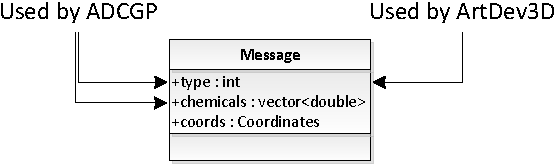
\includegraphics[scale=0.9]{diagram_ndevframe_msg-comparison}
	\caption{ADCGP vs. ArtDev3D: Use of messages}
	\label{fig:diagram_ndevframe_msg-comparison}
\end{figure}

Because the framework enforces use of common yet generic definitions of concepts, we can easily spot their differences. As with the example here, we clearly see that the difference between the two models is the fact that only one model uses chemicals when exchanging information. In fact, that is one of the reasons why chemicals have been reported to complicate things. If everything else had been the same, we could definitely say that this was the cause.


\subsection{Stability}
From the results we've seen so far, there are a number of things that can be said about these models. Most prominently, we see that ArtDev3D is able to evolve perfect specimens within relatively short time. With the sphere experiment, perfect fitness was achieved within just 500 generations. What can't be seen from the results is that it would achieve this typically within 50 generations! In contrast, the ADCGP model requires a lot of generations in order to reach higher fitness. At 10 000 generations, fitness rarely exceeded 0.9. Even when doubling that number, the population was still improving. Obviously, one cannot set it to run forever. The problem seemed to lie in the development method used in the models.

In ArtDev3D, the development or growth would stop after a certain amount of steps regardless of how long the development time. This ensures that the organisms will grow to target shape without overgrowing. H{\o}ye demonstrated this property in his thesis\cite{hoye2006}, and this is reflected by the model's ability to achieve high fitness fast. From the results obtained, it seemed that it is difficult to correctly evolve desired phenotype without knowing how many development steps will be needed. For instance, with the French flag experiment, using four development steps was optimal compared to three or five. Three was obviously not enough because the cells do not have the time to grow properly, while five was too much because the cells started to ``deform''. The new test showed this tendency as well, but it is difficult to state anything for certain with these results. As I've mentioned, one will have to develop a tool to look into each development step to ascertain this behaviour.
